\section{Result}

\subsection{Measurements for spring constant}

First we get the raw length measurement data in Table \ref{s1}.
\begin{table}[H]
	\centering
	\begin{tabular}{|p{0.7cm}|p{3cm}||p{0.7cm}|p{3cm}||p{0.7cm}|p{3cm}|}
	\hline
	\multicolumn{2}{|c|}{spring 1 [cm] $\pm$ 0.01 [cm]} &
	\multicolumn{2}{|c|}{spring 2 [cm] $\pm$ 0.01 [cm]} &
	\multicolumn{2}{|c|}{serial   [cm] $\pm$ 0.01 [cm]} \\ \hline
	$L_0$ & 0.00  & $L_0$ & 0.00  & $L_0$ & 20.00 \\ \hline
	$L_1$ & 2.00  & $L_1$ & 2.01  & $L_1$ & 23.96 \\ \hline
	$L_2$ & 3.96  & $L_2$ & 4.00  & $L_2$ & 27.94 \\ \hline
	$L_3$ & 5.96  & $L_3$ & 6.03  & $L_3$ & 31.90 \\ \hline
	$L_4$ & 8.02  & $L_4$ & 8.06  & $L_4$ & 36.40 \\ \hline
	$L_5$ & 10.04 & $L_5$ & 10.08 & $L_5$ & 39.94 \\ \hline
	$L_6$ & 12.02 & $L_6$ & 12.10 & $L_6$ & 44.02 \\ \hline
	\end{tabular}
	\caption{Spring constant measurement data}
	\label{s1}
\end{table}

Then we can calculate the change amount of the spring length by $\Delta L_i=L_i-L_0$ and get Table \ref{s2}.

\begin{table}[H]
	\centering
	\begin{tabular}{|p{0.7cm}|p{3cm}||p{0.7cm}|p{3cm}||p{0.7cm}|p{3cm}|}
	\hline
	\multicolumn{2}{|c|}{spring 1 [cm] $\pm$ 0.01 [cm]} &
	\multicolumn{2}{|c|}{spring 2 [cm] $\pm$ 0.01 [cm]} &
	\multicolumn{2}{|c|}{serial   [cm] $\pm$ 0.01 [cm]} \\ \hline
	$\Delta L_1$ & 2.00  & $\Delta L_1$ & 2.01  & $\Delta L_1$ & 3.96  \\ \hline
	$\Delta L_2$ & 3.96  & $\Delta L_2$ & 4.00  & $\Delta L_2$ & 7.94  \\ \hline
	$\Delta L_3$ & 5.96  & $\Delta L_3$ & 6.03  & $\Delta L_3$ & 11.90 \\ \hline
	$\Delta L_4$ & 8.02  & $\Delta L_4$ & 8.06  & $\Delta L_4$ & 16.40 \\ \hline
	$\Delta L_5$ & 10.04 & $\Delta L_5$ & 10.08 & $\Delta L_5$ & 19.94 \\ \hline
	$\Delta L_6$ & 12.02 & $\Delta L_6$ & 12.10 & $\Delta L_6$ & 24.02 \\ \hline
	\end{tabular}
	\caption{Calculated Spring constant measurement data}
	\label{s2}
\end{table}

We get the mass of the weight object for every $\Delta L_i$ in Table
\ref{massofweight}.

Since the acceleration due to gravity in Shanghai is $9.794 m/s^2$, we calculated
the weights of each weight object from its mass, as shown in Table
\ref{gravityofweight}. 

\begin{minipage}{0.5\linewidth}
	\begin{table}[H]
	\centering
	\begin{tabular}{|c|c|}
	\hline
	\multicolumn{2}{|c|}{m [g] $\pm$ 0.01 [g]} \\ \hline
	1 & 4.65  \\ \hline
	2 & 9.32  \\ \hline
	3 & 14.17 \\ \hline
	4 & 18.99 \\ \hline
	5 & 23.80 \\ \hline
	6 & 28.51 \\ \hline
	\end{tabular}
	\caption{Mass measurement data.}
	\label{massofweight}
	\end{table}
\end{minipage}
%
\begin{minipage}{0.5\linewidth}
	\begin{table}[H]
	\centering
	\begin{tabular}{|c|c|}
	\hline
	\multicolumn{2}{|c|}{F [N] $\pm$ 0.0001 [N]} \\ \hline
	1  & 0.0455  \\ \hline 
	2  & 0.0913  \\ \hline 
	3  & 0.1388  \\ \hline 
	4  & 0.1860  \\ \hline 
	5  & 0.2331  \\ \hline 
	6  & 0.2792  \\ \hline 
	\end{tabular}
	\caption{Weight measurement data.}
	\label{gravityofweight}
	\end{table}
\end{minipage}


% =====================================
% NOTE: Spring 1
For Spring 1, we can have its length change data versus the force affected on it
data.  

\begin{table}[H]
	\centering
	\begin{tabular}{|c|c|c|}
	\hline
	No. & length [cm] $\pm$ 0.01 [cm] & F [N] $\pm$ 0.0001 [N] \\ \hline
	$\Delta L_1$ & 2.00  &  0.0455  \\ \hline
	$\Delta L_2$ & 3.96  &  0.0913  \\ \hline
	$\Delta L_3$ & 5.96  &  0.1388  \\ \hline
	$\Delta L_4$ & 8.02  &  0.1860  \\ \hline
	$\Delta L_5$ & 10.04 &  0.2331  \\ \hline
	$\Delta L_6$ & 12.02 &  0.2792  \\ \hline
	\end{tabular}
	\caption{$\Delta L$  vs. Force for Spring 1}
	\label{s1df}
\end{table}

Then we use MATLAB fit tools to find $k_1$

\begin{figure}[H]
	\centering
	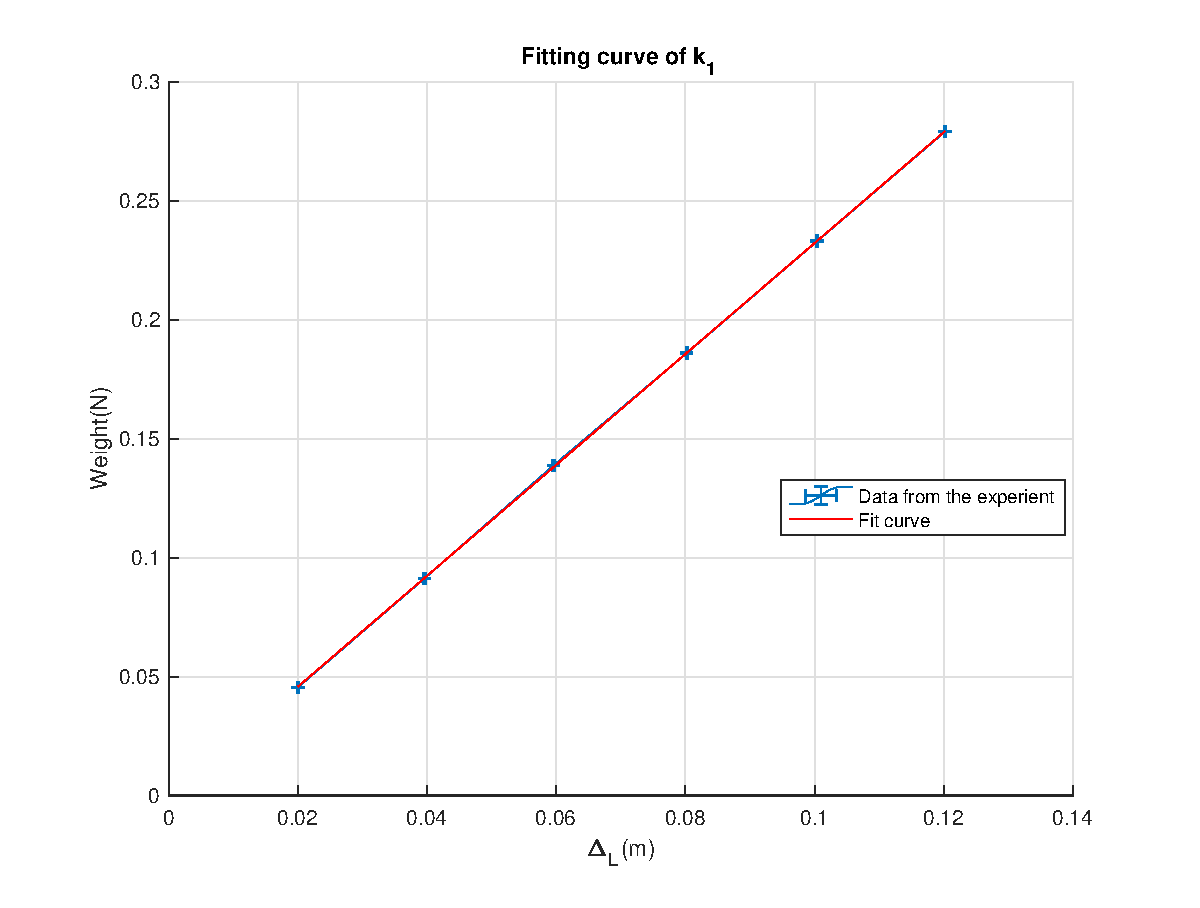
\includegraphics[width=15cm]{matlab/fitfig/k1}
	\caption{Fit curve of spring 1}
\end{figure}

$$ k_1 = 2.3311 \pm 0.013 [N/m] $$
$$ u_{k_1,r} = 0.55 \% $$

Goodness of fit:
\begin{quote}
	\centering
	SSE: 6.091e-07\\
	R-square: 1\\
	Adjusted R-square: 1 \\
	RMSE: 0.0003902 \\
\end{quote}


% =====================================
% NOTE: Spring 2
For Spring 2, we can have its length change data versus the force affected on it
data.  

\begin{table}[H]
	\centering
	\begin{tabular}{|c|c|c|}
	\hline
	No. & length [cm] $\pm$ 0.01 [cm] & F [N] $\pm$ 0.0001 [N] \\ \hline
	$\Delta L_1$ & 2.01  &  0.0455  \\ \hline
	$\Delta L_2$ & 4.00  &  0.0913  \\ \hline
	$\Delta L_3$ & 6.03  &  0.1388  \\ \hline
	$\Delta L_4$ & 8.06  &  0.1860  \\ \hline
	$\Delta L_5$ & 10.08 &  0.2331  \\ \hline
	$\Delta L_6$ & 12.10 &  0.2792  \\ \hline
	\end{tabular}
	\caption{$\Delta L$  vs. Force for Spring 2}
	\label{s2df}
\end{table}

Then we use MATLAB fit tools to find $k_2$

\begin{figure}[H]
	\centering
	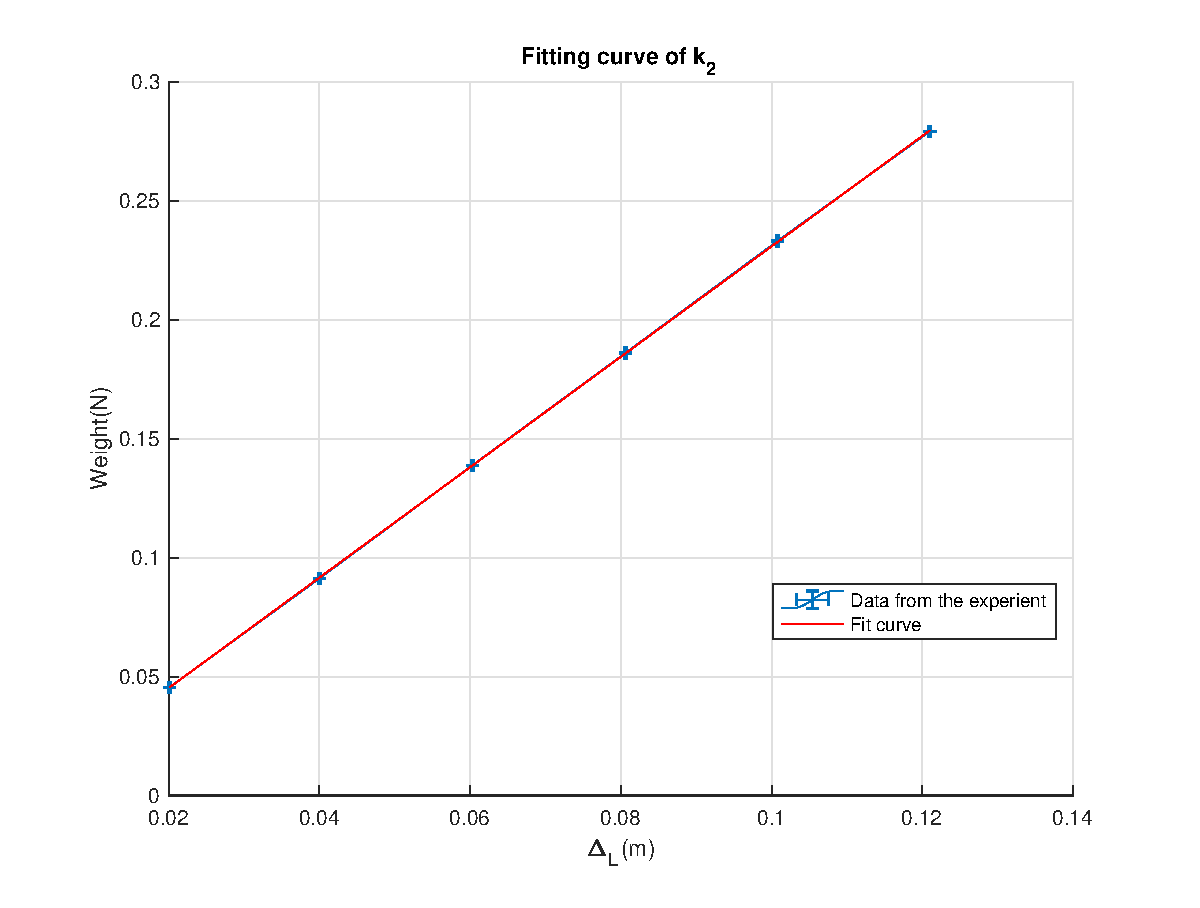
\includegraphics[width=15cm]{matlab/fitfig/k2}
	\caption{Fit curve of spring 2}
\end{figure}

$$k_2 =  2.3206 \pm 0.0105 [N/m] $$
$$ u_{k_2,r} = 0.45 \% $$

Goodness of fit:
\begin{quote}
	\centering
	SSE: 4.305e-07 \\
	R-square: 1 \\
	Adjusted R-square: 1 \\
 	RMSE: 0.0003281 \\
\end{quote}

% =====================================
% NOTE: Spring serial
For serial, we can have its length change data versus the force affected on it
data.  

\begin{table}[H]
	\centering
	\begin{tabular}{|c|c|c|}
	\hline
	No. & length [cm] $\pm$ 0.01 [cm] & F [N] $\pm$ 0.0001 [N] \\ \hline
	$\Delta L_1$ & 3.96  &  0.0455  \\ \hline
	$\Delta L_2$ & 7.94  &  0.0913  \\ \hline
	$\Delta L_3$ & 11.90 &  0.1388  \\ \hline
	$\Delta L_4$ & 16.40 &  0.1860  \\ \hline
	$\Delta L_5$ & 19.94 &  0.2331  \\ \hline
	$\Delta L_6$ & 24.02 &  0.2792  \\ \hline
	\end{tabular}
	\caption{$\Delta L$  vs. Force for serial}
	\label{ssdf}
\end{table}

Then we use MATLAB fit tools to find $k_3$ , in other words, the $k$ of the serial string.

\begin{figure}[H]
	\centering
	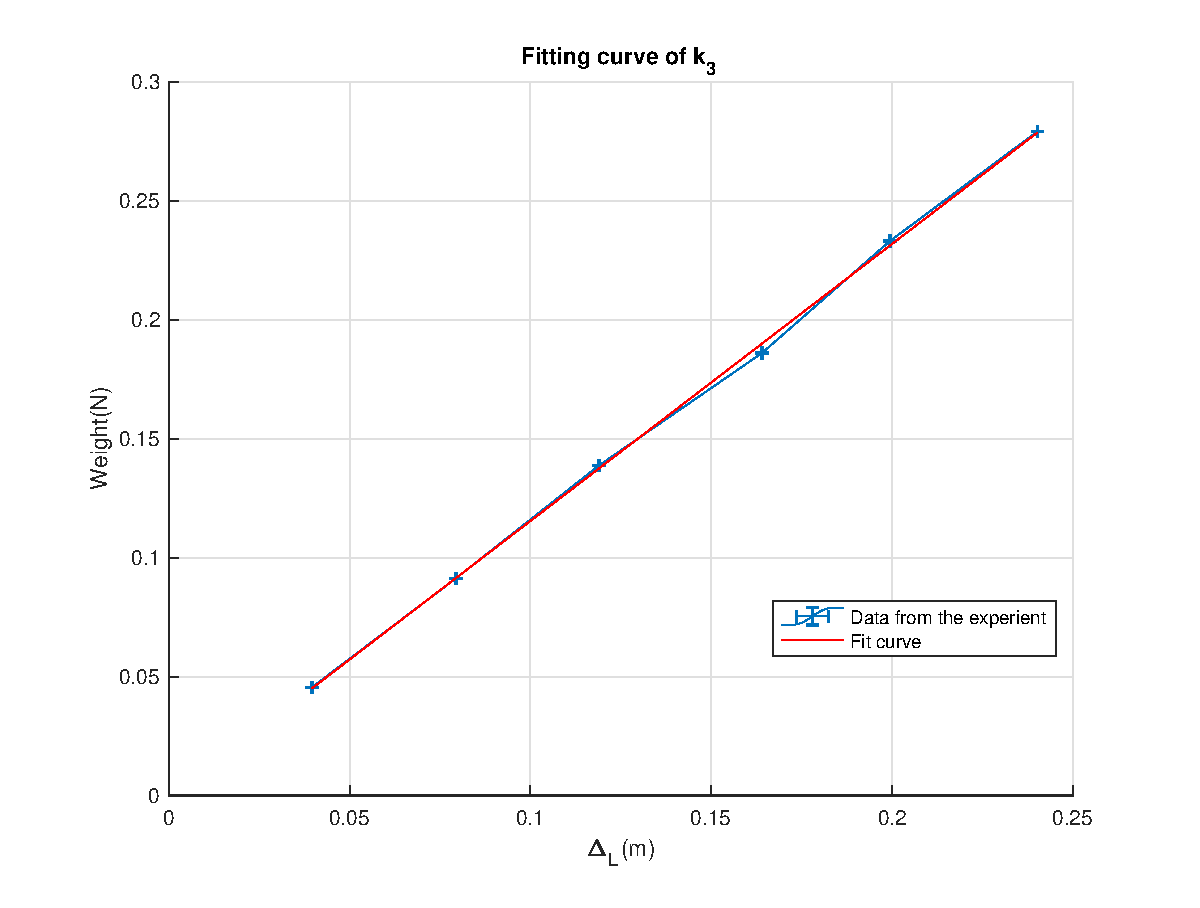
\includegraphics[width=15cm]{matlab/fitfig/k3}
	\caption{Fit curve of spring serial}
\end{figure}

$$k_3 = 1.165 \pm 0.0380 [N/m] $$
$$ u_{k_3,r} = 3.26 \% $$

Goodness of fit:
\begin{quote}
	\centering
	SSE: 2.144e-05
	R-square: 0.9994
	Adjusted R-square: 0.9993
	RMSE: 0.002315 
\end{quote}

% NOTE: k cal

By theory, we can calculate $k_3$, i.e. the $k$ of the spring serial by 
$$ k_{3,theory} = \frac{k_1 \cdot k_2 }{k_1 + k_2} =  1.1629 $$ 

Compared with $k_3 = 1.1649$  from the experiment,
$$ u_{k_{3,theory},k_3} = \frac{1.1649 - 1.1629}{1.1629} \cdot 100 \%  = 0.17 \% $$ 
The theory data is close to the experiment data
